% =====================================================================
%  ZipCount -- ICASSP 2027 version (4 pages content + 1 page references)
%  Compile: pdflatex main_icassp && bibtex main_icassp && pdflatex x2
%  Needs: texlive-publishers (IEEEtran), texlive-pictures (tikz)
%  Companion long version: main_taslp.tex
% =====================================================================
\documentclass[10pt,conference]{IEEEtran}
\IEEEoverridecommandlockouts

\usepackage{amsmath,amssymb}
\usepackage{booktabs}
\usepackage{tikz}
\usetikzlibrary{arrows.meta,positioning}
\usepackage[hidelinks]{hyperref}

\newcommand{\best}[1]{\textbf{#1}}
\newcommand{\sys}{ZipCount}

\begin{document}

\title{Low-Latency Streaming Speaker Counting\\with a Frozen ASR Encoder}
\author{\IEEEauthorblockN{Anonymous Submission}
\IEEEauthorblockA{Affiliation \\ email@domain}}
\maketitle

\begin{abstract}
Frame-level speaker counting underpins overlap-aware transcription and
turn-taking control, but is usually obtained from diarization systems that
are offline or operate at multi-second latency. We present \sys{}, which
emits a 4-way ordinal count $\{0,1,2,3^{+}\}$ every $640$\,ms with no
lookahead by freezing a public streaming Zipformer ASR encoder and training
only a $1.28$\,M-parameter causal decoder ($2\%$ of the model). Because
published counting numbers are rarely comparable, we re-score six system
configurations under one protocol -- identical windows, identical
$100$\,Hz rasterization, a common-window restriction -- on four corpora,
and report \sys{} as the mean of 3 independently trained seeds (std
$0.002$). At $640$\,ms \sys{} comes within $0.004$ mean macro-F1 of
NVIDIA's Sortformer-streaming running at its own $15.1$\,s budget, and
exceeds it by $0.028$ at matched latency, an offline Sortformer by $0.014$
and pyannote.audio~3.1 by $0.040$. A heavier offline WavLM pipeline stays
ahead, and we report the corpus where \sys{} ranks last. \sys{} runs at
$\mathrm{RTF}=0.08$ on one CPU thread.
\end{abstract}

\begin{IEEEkeywords}
speaker counting, overlapped speech detection, streaming, diarization
\end{IEEEkeywords}

% =====================================================================
\section{Introduction}

How many people are speaking in each frame is a compact but consequential
signal: it gates overlap-aware ASR, drives barge-in logic, and is what
overlapped speech detection (OSD) reports in binary form. Unlike full
diarization it needs no speaker identity, no clustering and no bounded
speaker inventory, which suits streaming deployment.

In practice counting is usually read off a diarization system. Clustering
pipelines~\cite{bredin2023pyannote,han2024diarizen} are offline by
construction. End-to-end neural diarization~\cite{fujita2019eend} and its
streaming descendants~\cite{liang2024fseend,liang2025lseend} relax this, and
NVIDIA's Sortformer~\cite{park2024sortformer} ships a streaming checkpoint
built on an arrival-order speaker cache~\cite{medennikov2025streamingsortformer}
-- whose default operating point, as we measure below, carries $15.1$\,s of
algorithmic latency. ``Streaming'' there means bounded memory, not real-time
response.

We invert the design order: fix the budget at $640$\,ms with zero lookahead,
then ask how much accuracy is attainable. Our answer reuses a frozen
streaming ASR encoder, which is already trained under the causal constraint
we need. Contributions: (i) a $640$\,ms streaming counter combining a frozen
Zipformer~\cite{yao2024zipformer} with a multi-scale hypercolumn, a
dev-selected fixed stack mask with a learned gated projection, and a causal
dual-dilation TCN; (ii) a unified re-scoring protocol, since window length
and frame rate silently change macro-F1;
(iii) a four-corpus comparison against two Sortformer configurations at two
latencies, an offline Sortformer and pyannote.audio, with DER context and
measured RTF; (iv) ablations including a negative result -- the stack choice
that improves frame accuracy measurably degrades temporal smoothness.

\textbf{Related work.} TCN-based detectors for OSD and counting on meeting
data are established~\cite{cornell2020osd,bullock2020overlap}, and
real-time counting has been addressed
directly~\cite{yousefi2021realtime}; those systems are typically non-causal
or binary, whereas we predict a 4-way ordinal count causally. LS-EEND
recovers a count via a termination marker~\cite{liang2025lseend}. Reusing
frozen ASR representations for speaker information also has
precedent~\cite{msaasr2024}. Our contribution is the instantiation under a
hard causal budget and the latency-controlled benchmark, not the frozen-head
pattern itself.

% =====================================================================
\section{Method}
\label{sec:method}

\begin{figure}[t]
\centering
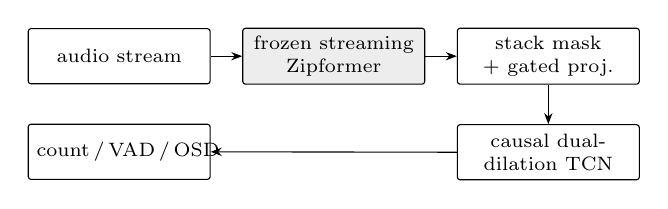
\begin{tikzpicture}[
  font=\scriptsize,
  box/.style={draw,rounded corners=1pt,align=center,inner sep=3pt,
              minimum height=7mm,text width=21mm},
  ar/.style={-{Stealth[length=1.4mm]}}]
\node[box] (a) {audio stream};
\node[box,right=4mm of a,fill=black!7] (z) {frozen streaming\\Zipformer};
\node[box,right=4mm of z] (s) {stack mask\\+ gated proj.};
\node[box,below=5mm of s] (t) {causal dual-\\dilation TCN};
\node[box,below=5mm of a] (h) {count\,/\,VAD\,/\,OSD};
\draw[ar] (a)--(z); \draw[ar] (z)--(s); \draw[ar] (s)--(t);
\draw[ar] (t.west)--(h.east);
\end{tikzpicture}
\caption{Only the two right-hand blocks are trained ($1.28$\,M of
$65.8$\,M parameters); output is $25$\,Hz, one block of $16$ frames every
$640$\,ms.}
\label{fig:arch}
\end{figure}

\textbf{Task.} The model emits at $25$\,Hz a distribution over
$c_t\!\in\!\{0,1,2,3^{+}\}$ in blocks of $16$ frames, one per $640$\,ms,
with no right context: lookahead $0$\,ms, chunking delay $640$\,ms worst
case, compute $20.7$\,ms, worst-case response $660.7$\,ms -- the budget we
write ``$640$\,ms'' for throughout.

\textbf{Frozen backbone.} We use the public LibriSpeech streaming
Zipformer~\cite{yao2024zipformer} ($64.56$\,M parameters), causal, chunk
size $32$, $128$ left-context frames, entirely frozen. Its encoder is
U-shaped: six stacks with downsampling $(1,2,4,8,4,2)$ and widths
$(192,\dots,256)$ run at different temporal resolutions.

\textbf{Hypercolumn and stack selection.} We resample every stack to
$25$\,Hz and concatenate ($1984$ dims). Each slice is LayerNorm-ed
separately -- their activation scales differ by an order of magnitude --
weighted by a softmax gate and projected to $d\!=\!192$. A fixed binary mask
$m\!\in\!\{0,1\}^{6}$ replaces masked slices by exact zero blocks after
their LayerNorm, so no masked \emph{feature} reaches the output while every
module, parameter count and seeded initialization stays identical across
mask settings; ablations are matched by construction. The gate is
deliberately not renormalized: masked gates absorb probability mass ($0.57$
in our trained model) but multiply zero blocks, so this is a global
rescaling that the following projection absorbs. Our system uses
$m=(1,1,1,0,0,0)$, the three highest-resolution stacks.

\textbf{Causal decoder.} An overlap is confirmed by seconds of evidence, but
its boundaries are frame-local. Six residual blocks with dilations
$1,\dots,32$ each run \emph{two} depthwise convolutions (kernel $3$) over
the same normalized input -- dilation $1$ for onset detail, dilation $d$ for
segment context -- concatenated through a GLU, so each block gates context
against detail per frame. Left-only padding gives a $127$-frame ($5.08$\,s)
causal receptive field. For streaming each block caches its last
$(k\!-\!1)d$ \emph{post}-normalization frames: \texttt{forward} pads after
the norm, so the initial cache must be literal zeros, whereas raw zeros
prepended before the norm become $\beta\!\neq\!0$ and perturb each stream's
first receptive field.

\textbf{Output and objective.} The head emits 4-way count logits plus
cumulative logits $P(c\!\geq\!1)$ (VAD) and $P(c\!\geq\!2)$ (OSD) from the
same trunk. The loss is
\begin{equation}
\mathcal{L}=\mathcal{L}^{\text{SORD}}_{\text{count}}
+\lambda_{\text{aux}}^{\top}\mathcal{L}_{\text{aux}}
+\lambda_{\text{reg}}^{\top}\mathcal{L}_{\text{reg}},
\end{equation}
where $\mathcal{L}^{\text{SORD}}$ uses soft ordinal
labels~\cite{diaz2019sord} ($\alpha\!=\!2.5$) with class weights
$(1,1,1.5,3)$; $\mathcal{L}_{\text{aux}}$ collects VAD ($0.3$), overlap
($0.5$), Dice ($0.5$), branch consistency ($0.2$) and monotonicity ($0.1$);
$\mathcal{L}_{\text{reg}}$ collects expected-MAE ($0.2$) and a
symmetric-KL temporal smoothness term ($0.02$).

% =====================================================================
\section{Experimental Setup}

\textbf{Training.} The head trains for $3000$ steps (batch $24$, Adam,
lr $10^{-3}$ cosine, $500$ warmup, AMP) on $253{,}452$ $30$\,s windows from
LibriMix~\cite{cosentino2020librimix} ($107.9$\,k),
AMI~\cite{carletta2005ami} ($39.5$\,k), NOTSOFAR-1 ($32.4$\,k), AliMeeting
($26.9$\,k), AISHELL-4 ($11.7$\,k), MSDWild~\cite{liu2022msdwild}
($8.6$\,k), RAMC ($6$\,k), VoxConverse~\cite{chung2020voxconverse}
($2.5$\,k) plus single-speaker, MUSAN~\cite{snyder2015musan} and silence
windows. Noise, RIR and gain augmentation are applied to the synthetic
portion only. Splits are disjoint, but AMI, VoxConverse and MSDWild are
\emph{in-domain} (their train splits are in the mix);
DipCo~\cite{vansegbroeck2020dipco} is never seen. Baselines have their own
overlapping training data, so no system here is domain-neutral.

\textbf{Unified protocol.} Counting scores depend sharply on two often
implicit choices: window length, which sets how much context an offline
system gets, and rasterization rate, which sets how boundary frames are
charged. We therefore re-score \emph{every} system, including ours, on
identical assets -- $90$\,s windows cut from the corpora's original
per-speaker RTTMs, rasterized at $100$\,Hz. \sys{}'s $25$\,Hz output is
upsampled $4\times$, charging it honestly for the $40$\,ms boundaries it
cannot place. All systems are restricted to the windows every system
produced output for. Diarization outputs become counts by summing active
tracks per frame with one shared rasterizer.

\textbf{Model selection.}
\label{sec:selection}
Every architecture decision reported here -- the decoder, the stack mask and
eight further candidates we rejected -- was made on one fixed development
set: a $116$-recording half of the VoxConverse test set. Loss weights and
the $3000$-step endpoint were fixed beforehand. No AMI, DipCo or MSDWild
material was inspected during selection, so those columns are untouched. We
exclude the development half from all reported numbers and score VoxConverse
only on the sealed complementary half ($964$ windows). The difference is
worth reporting: moving to the sealed half costs \sys{} $0.021$ macro-F1,
the largest shift of any system, while the five untuned baselines move by
$-0.013$ to $+0.024$. A single-corpus development set is a real limitation
of this study.

\textbf{Systems.} DiariZen~\cite{han2024diarizen} (WavLM-Large~\cite{chen2022wavlm}
+ clustering, offline); Sortformer-offline (\texttt{4spk-v1})~\cite{park2024sortformer};
Sortformer-streaming (\texttt{4spk-v2.1})~\cite{medennikov2025streamingsortformer}
at its released default (chunk
$188$, right context $1$; $15{,}120$\,ms) and at chunk $8$, right context
$0$ ($640$\,ms) -- the latter \emph{off-label}, below the model's trained
operating point, reported as a latency-matched reference rather than a
vendor setting; pyannote.audio~3.1~\cite{bredin2023pyannote}, taking the
overlap-preserving output.

% =====================================================================
\section{Results}
\label{sec:results}

\begin{table}[t]
\centering
\caption{Macro-F1, unified protocol, corpora weighted equally.
$^{\dagger}$in-domain for \sys{}. $^{*}$off-label. $^{\ddagger}$mean of 3
seeds, std $0.002$.}
\label{tab:main}
\footnotesize
\setlength{\tabcolsep}{2.6pt}
\begin{tabular}{lccccc c}
\toprule
System & Lat. & AMI$^{\dagger}$ & DipCo & VoxC.$^{\dagger}$ & MSDW.$^{\dagger}$ & Mean \\
\midrule
DiariZen              & off.       & \best{.765} & .495 & .656 & \best{.642} & \best{.640} \\
Sortf.-str.\ (def.)   & 15.1\,s    & .564 & .518 & \best{.680} & .554 & .579 \\
\sys{} (ours)$^{\ddagger}$ & \best{640\,ms} & .654 & \best{.552} & .542 & .553 & .575 \\
Sortf.-offline        & off.       & .606 & .501 & .624 & .513 & .561 \\
Sortf.-str.$^{*}$     & 640\,ms    & .539 & .495 & .616 & .537 & .547 \\
pyannote 3.1          & off.       & .594 & .464 & .574 & .509 & .535 \\
\bottomrule
\end{tabular}
\end{table}

\textbf{Cross-corpus comparison.} DiariZen wins clearly ($0.640$), ahead of
everything else by more than $0.06$. The meaningful axis is latency:
\sys{} ($0.575$, mean of 3 seeds) comes within $0.004$ of
Sortformer-streaming at $1/23$ of its budget, and at matched $640$\,ms
leads it by $0.028$, Sortformer-offline by $0.014$ and pyannote by $0.040$
-- the latter two consuming whole utterances. Against DiariZen the gap is
real: a frozen $1.28$\,M-parameter causal head does not replace a
fine-tuned WavLM pipeline with global clustering.

We test these differences with a paired bootstrap ($10{,}000$ resamples,
\sys{}'s per-window confusions pooled over the same 3 seeds as
Table~\ref{tab:main}) that resamples recordings \emph{within} each corpus
and averages macro-F1 over corpora with equal weight, reproducing exactly
the quantity in Table~\ref{tab:main}; recordings are the unit because
windows from one recording are not independent draws. This measures the
sampling variance of the \emph{difference between two fixed systems}, not
the seed-to-seed variance of retraining one, which we measured directly at
$0.002$ (std, 3 seeds) -- an order of magnitude below every resolved gap
below. Taking $\Delta$ positive in \sys{}'s favour: DiariZen $-0.065$, CI
$[-0.074,-0.054]$; Sortformer-streaming at its $15.1$\,s default $-0.004$,
CI $[-0.016,+0.008]$, $p\!=\!0.58$; Sortformer-offline $+0.014$,
$[+0.004,+0.024]$, $p\!=\!0.007$; the same streaming checkpoint at
$640$\,ms $+0.028$, $[+0.017,+0.039]$; pyannote $+0.040$,
$[+0.029,+0.047]$. The comparison against Sortformer-streaming at its own
budget is therefore \emph{not resolved} -- the two are indistinguishable on
this evidence while \sys{} runs $23\times$ faster to first output -- whereas
at matched latency \sys{}'s lead is clear. The advantage over
Sortformer-offline is narrower than the others, though the interval clears
zero.

Behaviour is not uniform, and the pattern runs against the obvious
objection. \sys{}'s only outright win is DipCo, the one corpus absent from
its training mix, while its only last place is VoxConverse, which is
in-domain: every system scores DER below $10\%$ there, its web-video clips
having cleaner turn-taking and $0$/$1$-dominated counts than our
meeting-heavy mix. \sys{}'s advantage concentrates in dense multi-party
overlap and erodes where overlap is rare.

\textbf{DER context.} For the five identity-emitting systems, mean DER
(collar $0.25$\,s, overlap included) is DiariZen $20.6\%$,
Sortformer-offline $22.6\%$, Sortformer-streaming $24.2\%$, pyannote
$25.8\%$ and Sortformer-streaming at $640$\,ms $28.3\%$ -- broadly tracking
the macro-F1 ordering, so the count rasterizer is not manufacturing it.
Latency can only be isolated \emph{within} a checkpoint, since the offline
and streaming Sortformers are different released models: reducing the
streaming model's latency to $640$\,ms costs $+4.1$ DER points and $-0.030$
macro-F1, the same direction in both metrics. \sys{} emits no speaker
identity, so DER is undefined for it.

\textbf{Compute.} With the production streaming loop (carried caches, batch
$1$), \sys{} needs $20.7$\,ms per $640$\,ms block on an RTX~3090
($\mathrm{RTF}\,{=}\,0.032$, p95 $21.9$\,ms) and $51.4$\,ms single-threaded
on an i7-12700 ($\mathrm{RTF}\,{=}\,0.080$, p95 $53.0$\,ms) -- over
$12\times$ headroom without a GPU. Extra CPU threads do not help
($51.7$\,ms): one batch-1 block offers too little intra-op parallelism, so
threads buy throughput across streams, not single-stream latency.

% =====================================================================
\section{Ablations}
\label{sec:ablation}

\begin{table}[t]
\centering
\caption{Stack selection, mean of 3 seeds. ``n.s.'' = below seed range.
Edit score higher-better; fragmentation best near $1.0$.}
\label{tab:ablation}
\small
\begin{tabular}{lccc}
\toprule
Metric / corpus & mask & all stacks & $\Delta$ \\
\midrule
macro-F1, AMI test        & 0.657 & 0.622 & $+0.035$ \\
macro-F1, DipCo eval      & 0.540 & 0.532 & $+0.008$ \\
macro-F1, VoxConverse     & 0.554 & 0.546 & $+0.009$ \\
macro-F1, MSDWild         & 0.552 & 0.548 & $+0.004$ (n.s.) \\
OSD-F1, VoxConverse       & 0.496 & 0.471 & $+0.025$ \\
\midrule
Edit score, VoxConverse   & 38.69 & 40.70 & $-2.01$ \\
Edit score, MSDWild       & 53.33 & 55.82 & $-2.49$ \\
Fragmentation, VoxConv.   & 3.21 & 3.06 & $+0.15$ (n.s.) \\
ECE, VoxConverse          & 0.111 & 0.106 & $+0.005$ (n.s.) \\
\bottomrule
\end{tabular}
\end{table}

\textbf{Stack selection trades smoothness for accuracy.}
Table~\ref{tab:ablation} holds parameter count, initialization and schedule
fixed across three seeds. Suppressing the three deep, heavily-downsampled
stacks improves frame accuracy consistently ($+0.035$ macro-F1 on AMI test;
$+0.025$ OSD-F1 on all three VoxConverse splits) -- and makes the output
measurably \emph{less} smooth. Across the four window-based evaluation sets,
segmental edit score falls by $1.86$--$2.49$ points and fragmentation rises,
consistent in direction everywhere (edit score exceeds seed range on three
of four). Calibration is unaffected. The deep stacks evidently supply
long-range consistency the $5.08$\,s receptive field does not replace;
discarding them buys per-frame accuracy at the cost of flicker.

\textbf{Decoder.} Replacing the dual-dilation TCN by a size-matched causal
deformable decoder ($1.32$ vs.\ $1.28$\,M), same training, three paired
seeds, costs $0.0022$ macro-F1 (bootstrap CI $[+0.0007,+0.0039]$ favouring
the TCN). Fragmentation falls $2.53\!\rightarrow\!2.36$ and boundary F1
rises $0.341\!\rightarrow\!0.350$ with overlap recall unchanged: deformable
sampling chooses \emph{where} to look but carries no bias toward
piecewise-constant output, which is the deficit dilated convolutions
address.

\textbf{Baselines and gate design.} Three parameter-matched, 3-seed arms
test whether the architecture is doing real work: a final-stack-only system
(mask $(0,0,0,0,0,1)$) scores $0.399$, $-0.176$ vs.\ \sys{} (CI
$[-0.185,-0.168]$); a from-scratch log-mel backbone (no ASR pretraining at
all, same TCN) scores $0.426$, $-0.149$ (CI $[-0.157,-0.141]$) -- and
notably \emph{beats} the final-stack arm, so a single deep stack of the
pretrained encoder is worse than no pretraining at all; renormalizing the
gate over active stacks only (instead of softmax over all six, masked
zeroed after) scores $0.544$, $-0.032$ (CI $[-0.038,-0.026]$) -- the
non-renormalized design optimizes better despite ``wasting'' $0.57$ of its
gate mass. All three gaps are resolved by paired bootstrap ($p<10^{-3}$).

\textbf{Fine-tuning is unstable.} Unfreezing the backbone is not reliably
beneficial: over five seeds and three learning rates
($10^{-5}$--$3\!\times\!10^{-5}$), two seeds degraded at \emph{every} rate
while three improved, and the spread across fine-tuning configurations
($0.022$--$0.052$) far exceeds head-only training ($0.0045$). This is
seed-structural, not a mis-tuned rate, and is why the frozen configuration
is our reported system.

% =====================================================================
\section{Conclusion}

\sys{} emits an ordinal speaker count every $640$\,ms with no lookahead,
training $2\%$ of its weights on top of a frozen streaming ASR encoder, and
is competitive with NVIDIA's streaming Sortformer at $1/23$ of its latency
while running at $\mathrm{RTF}=0.08$ on a single CPU thread (Table~\ref{tab:main}).
A heavier offline pipeline remains ahead, and one sparse-overlap corpus
exposes a genuine weakness. Ablations show the stack choice improving frame
accuracy simultaneously degrades segment smoothness -- hidden from a
frame-level metric alone -- and that three architectural alternatives
(final Zipformer stack only, no pretraining at all, a renormalized gate)
each cost $0.03$--$0.18$ macro-F1, resolved by paired bootstrap: the
multi-scale hypercolumn and the gate's exact form are not incidental
choices.

\bibliographystyle{IEEEtran}
\bibliography{refs}
\end{document}
